% =============================================================================
%  TPF -- IA aplicada a la Robótica
%  Presentación de 10 minutos, para exponer ante profesores y compañeros.
%  14 diapositivas (unos 9 minutos) + 5 de respaldo para las preguntas.
%
%  Compilar (dos pasadas):   pdflatex TPF_presentacion.tex
%
%  El guion, con el tiempo y lo que se dice en cada diapositiva, está en
%  GUION.md. El video para proyectar es demo_vista_del_robot.mp4 (20 s).
%
%  OJO al editar: el cuerpo de un frame no puede empezar con una llave "{":
%  beamer la toma como subtítulo y el contenido desaparece sin dar error.
% =============================================================================
\documentclass[aspectratio=169,11pt]{beamer}

\usetheme{metropolis}
\usepackage[T1]{fontenc}
\usepackage[utf8]{inputenc}
\usepackage[spanish,es-noquoting]{babel}
\usepackage{tikz}
\usetikzlibrary{positioning,arrows.meta,fit,backgrounds,calc}
\usepackage{booktabs}
\usepackage{amsmath}
\usepackage{array}
\usepackage{xcolor}
\usepackage{graphicx}
\usepackage{microtype}
\DisableLigatures{encoding = T1, family = tt*}

\graphicspath{{figuras/}}

\definecolor{azul}{HTML}{2A78D6}
\definecolor{naranja}{HTML}{EB6834}
\definecolor{gris}{HTML}{52514E}
\definecolor{grisclaro}{HTML}{898781}
\definecolor{critico}{HTML}{D03B3B}
\definecolor{verde}{HTML}{0CA30C}
\definecolor{ambar}{HTML}{FAB219}

\setbeamercolor{frametitle}{bg=azul}
\setbeamercolor{progress bar}{fg=naranja}
\setbeamercolor{alerted text}{fg=critico}
\setbeamertemplate{frame numbering}[fraction]
\metroset{block=fill}
\setbeamersize{text margin left=8mm, text margin right=8mm}
\setlength{\tabcolsep}{5pt}

\newcommand{\hacia}{$\rightarrow$}
\newcommand{\grad}{\ensuremath{^\circ}}
\newcommand{\destaca}[1]{\textcolor{azul}{\textbf{#1}}}
\newcommand{\ojo}[1]{\textcolor{critico}{\textbf{#1}}}
\newcommand{\cod}[1]{\texttt{\detokenize{#1}}}
\newcolumntype{L}[1]{>{\raggedright\arraybackslash}p{#1}}
% Una imagen de la tira, con su leyenda debajo.
\newcommand{\cuadro}[2]{%
  \begin{column}{0.19\textwidth}
    \centering
    \includegraphics[width=\textwidth]{#1}\\[2pt]
    {\footnotesize #2}
  \end{column}}

\title{Un robot que busca y huye}
\subtitle{Aproximación y evasión con visión por IA a bordo}
\author{Federico Morán}
\institute{Trabajo Práctico Final --- IA aplicada a la Robótica \\
           Maestría en Inteligencia Artificial}
\date{Octubre de 2026}

\begin{document}

\maketitle

% ----------------------------------------------------------------------- 2
\begin{frame}{El problema}
  \begin{alertblock}{}
    \centering\large
    Un robot que \textbf{recorre una sala}, \textbf{reconoce dos objetos con la
    cámara} y \textbf{reacciona distinto} ante cada uno.
  \end{alertblock}

  \vspace{0.2em}
  \begin{columns}[T,onlytextwidth]
    \begin{column}{0.27\textwidth}
      \centering
      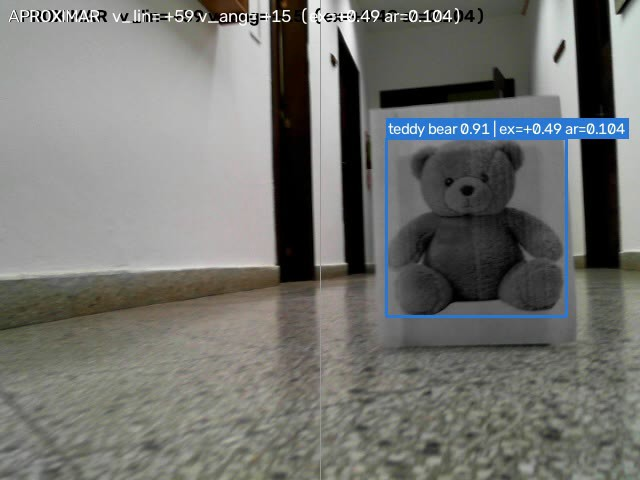
\includegraphics[width=\textwidth]{oso_3.jpg}\\[3pt]
      \textcolor{azul}{\textbf{Oso}}: \textbf{se acerca}
    \end{column}
    \begin{column}{0.27\textwidth}
      \centering
      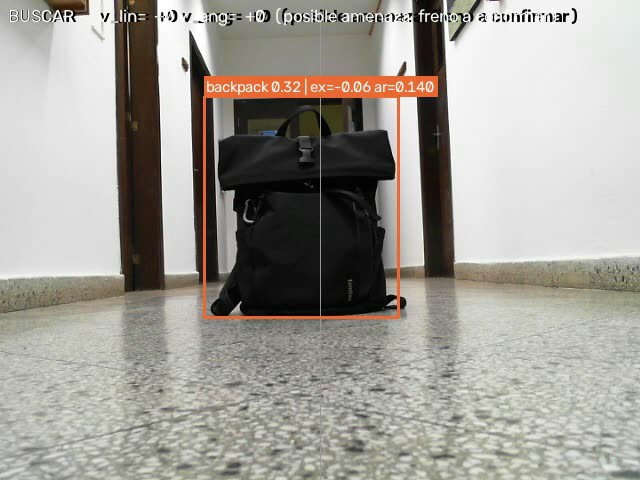
\includegraphics[width=\textwidth]{huir_1.jpg}\\[3pt]
      \textcolor{naranja}{\textbf{Mochila}}: \textbf{huye}
    \end{column}
    \begin{column}{0.40\textwidth}
      \begin{itemize}
        \item Si ve los dos, \textbf{huir gana}.
        \item Todo se decide \textbf{a bordo}: sin PC externa, sin
              teleoperación, sin nube.
      \end{itemize}

      {\footnotesize\textcolor{grisclaro}{Las imágenes son de la cámara del
      robot, con lo que detecta la red.}}
    \end{column}
  \end{columns}
\end{frame}

% ----------------------------------------------------------------------- 3
\begin{frame}{El robot}
  \begin{columns}[c,onlytextwidth]
    \begin{column}{0.47\textwidth}
      \centering
      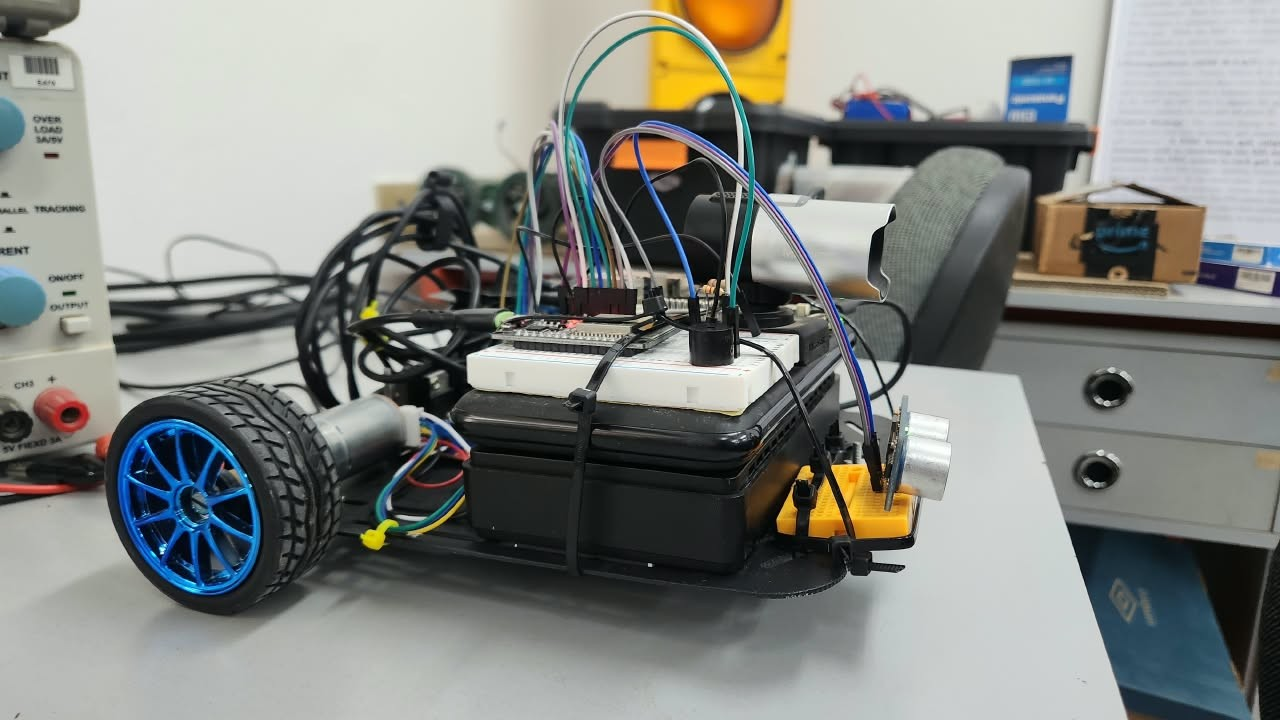
\includegraphics[width=\textwidth]{robot_terminado.jpg}\\[3pt]
      {\footnotesize\textcolor{grisclaro}{El robot terminado, el 2 de octubre.}}
    \end{column}
    \begin{column}{0.50\textwidth}
      \small
      \begin{itemize}
        \item \textbf{Raspberry Pi 5} --- ve y decide.
        \item \textbf{ESP32} --- mueve los motores y protege.
        \item \textbf{Webcam USB} y \textbf{ultrasónico} al frente.
        \item \textbf{Driver L298N} y dos motores de 12 V con reductora.
        \item \textbf{Buzzer}: avisa cuando huye y cuando llega.
        \item \textbf{Dos baterías separadas}: una para el Pi, otra para los
              motores.
        \item \textbf{Tracción diferencial}: dos ruedas motrices y una rueda
              loca; gira dándole distinta velocidad a cada rueda.
      \end{itemize}
    \end{column}
  \end{columns}
\end{frame}

% ----------------------------------------------------------------------- 4
\begin{frame}{Arquitectura: dos niveles}
  \centering
  \begin{tikzpicture}[font=\small, >={Stealth[length=2.2mm]},
      b/.style={draw, rounded corners=2pt, minimum height=1.0cm, align=center,
                line width=0.9pt, text width=2.15cm, inner sep=2pt}]
    \node[b, draw=azul, fill=azul!8] (cam) {Cámara};
    \node[b, draw=azul, fill=azul!8, right=0.4cm of cam] (yolo) {Red neuronal\\YOLOv8n};
    \node[b, draw=azul, fill=azul!8, right=0.4cm of yolo] (est) {Máquina de\\estados};
    \node[b, draw=azul, fill=azul!8, right=0.4cm of est] (ctl) {Ley de\\control};
    \begin{scope}[on background layer]
      \node[draw=azul, dashed, rounded corners=4pt, fit=(cam)(ctl), inner sep=8pt,
            label={[azul]above:\textbf{Raspberry Pi 5 --- decide, 11 veces por segundo}}] {};
    \end{scope}
    \node[b, draw=naranja, fill=naranja!8, below=1.6cm of ctl] (par) {Calibración\\por rueda};
    \node[b, draw=naranja, fill=naranja!8, left=0.4cm of par] (pwm) {PWM};
    \node[b, draw=gris, fill=gris!8, left=0.4cm of pwm] (mot) {Driver y\\motores};
    \node[b, draw=naranja, fill=naranja!8, left=0.4cm of mot] (wd) {Freno\\automático};
    \begin{scope}[on background layer]
      \node[draw=naranja, dashed, rounded corners=4pt, fit=(par)(pwm)(wd), inner sep=8pt,
            label={[naranja]below:\textbf{ESP32 --- ejecuta, 100 veces por segundo}}] {};
    \end{scope}
    \draw[->] (cam) -- (yolo); \draw[->] (yolo) -- (est); \draw[->] (est) -- (ctl);
    \draw[->, line width=1.2pt] (ctl) -- node[left, pos=0.38]{``avanzá tanto, girá tanto''} (par);
    \draw[->] (par) -- (pwm); \draw[->] (pwm) -- (mot);
    \draw[->] (wd) -- (mot);
  \end{tikzpicture}

  \vspace{0.1em}
  \small
  El Pi \textbf{nunca toca un motor}; el ESP32 \textbf{nunca decide}: mueve,
  mide la distancia con el ultrasónico y hace sonar el buzzer. Si el Pi deja
  de hablar medio segundo, el ESP32 \textbf{frena solo}.
\end{frame}

% ----------------------------------------------------------------------- 5
\begin{frame}{La IA: detección de objetos a bordo}
  \begin{columns}[c,onlytextwidth]
    \begin{column}{0.44\textwidth}
      \centering
      % Barras horizontales: una por tamaño de imagen, de arriba hacia abajo.
      \begin{tikzpicture}[font=\footnotesize, x=0.27cm, y=0.78cm]
        \draw[gris, line width=0.8pt] (0,-0.5) -- (0,3.6);
        \foreach \y/\v/\t/\c in {3/3.2/640 px/grisclaro, 2/5.2/480 px/grisclaro, 1/11.3/320 px/azul, 0/17.7/256 px/grisclaro} {
          \fill[color=\c] (0,\y-0.3) rectangle (\v,\y+0.3);
          \node[left] at (0,\y) {\t};
        }
        \node[white, left] at (3.3,3) {\textbf{3,2}};
        \node[white, left] at (5.3,2) {\textbf{5,2}};
        \node[white, left] at (11.4,1) {\textbf{11,3}};
        \node[white, left] at (17.8,0) {\textbf{17,7}};
        \draw[critico, dashed, line width=1pt] (5,-0.5) -- (5,3.75);
        \node[critico, above] at (5,3.7) {mínimo aceptable: 5};
        \node[below] at (9,-0.5) {imágenes por segundo};
        \node[azul, right] at (11.5,1) {\textbf{elegido}};
      \end{tikzpicture}
    \end{column}
    \begin{column}{0.53\textwidth}
      \begin{itemize}
        \item \textbf{YOLOv8n}, preentrenada en COCO (80 clases). Sin
              entrenamiento propio.
        \item Se midió el compromiso: a \textbf{320 px, 11 imágenes por
              segundo} en la Raspberry Pi 5.
        \item De la foto a la decisión: \textbf{$\sim$150 ms}.
        \item Una detección aislada no alcanza: hacen falta \textbf{3 imágenes
              seguidas} para creerle.
      \end{itemize}
    \end{column}
  \end{columns}

  \vspace{0.4em}
  \small
  El aporte no es entrenar una red: es \destaca{meter la inferencia dentro de
  un lazo de control físico} que corre en tiempo real.
\end{frame}

% ----------------------------------------------------------------------- 6
\begin{frame}{El comportamiento: cuatro estados y una prioridad}
  \centering
  \begin{tikzpicture}[font=\small, >={Stealth[length=2.2mm]},
      e/.style={draw, rounded corners=3pt, minimum height=1.6cm, text width=2.85cm,
                align=center, line width=1pt}]
    \node[e, draw=gris, fill=gris!8] (b) {\textbf{BUSCAR}\\{\footnotesize mira quieto,}\\{\footnotesize gira un paso}};
    \node[e, draw=azul, fill=azul!8, right=1.9cm of b] (a) {\textbf{APROXIMAR}\\{\footnotesize avanza y}\\{\footnotesize centra el oso}};
    \node[e, draw=verde, fill=verde!8, right=1.9cm of a] (f) {\textbf{ENCONTRADO}\\{\footnotesize frena a}\\{\footnotesize $\sim$30 cm}};
    \node[e, draw=naranja, fill=naranja!12, below=1.4cm of a] (h) {\textbf{HUIR}\\{\footnotesize retrocede, gira}\\{\footnotesize y se aleja}};
    \draw[->, line width=1pt] ([yshift=5pt]b.east) -- node[above]{ve el oso} ([yshift=5pt]a.west);
    \draw[->, line width=1pt] ([yshift=-5pt]a.west) -- node[below]{lo pierde} ([yshift=-5pt]b.east);
    \draw[->, line width=1pt] (a) -- node[above]{llegó} (f);
    \draw[->, naranja, line width=1.2pt] (b.south) |- node[pos=0.25, left]{mochila} (h.west);
    \draw[->, naranja, line width=1.2pt] ([xshift=12pt]a.south) -- node[right]{mochila} ([xshift=12pt]h.north);
    \draw[->, naranja, line width=1.2pt] (f.south) |- node[pos=0.25, right]{mochila} (h.east);
    \draw[->, gris, dashed, line width=1pt] ([xshift=-30pt]h.north) -- ++(0,0.75) -| node[pos=0.22, above]{terminó de huir} ([xshift=16pt]b.south);
  \end{tikzpicture}

  \vspace{0.6em}
  \small
  \textcolor{naranja}{\textbf{La mochila interrumpe cualquier estado}}: la
  conducta de seguridad siempre gana. Y con algo a menos de 30 cm adelante,
  \textbf{no avanza: gira}. Todo se verificó \textbf{sin robot}, con 79
  pruebas automáticas.
\end{frame}

% ----------------------------------------------------------------------- 7
\begin{frame}{El control: de una caja en la imagen a dos velocidades}
  \begin{columns}[c,onlytextwidth]
    \begin{column}{0.42\textwidth}
      \centering
      \begin{tikzpicture}[font=\footnotesize, x=0.82cm, y=0.82cm]
        \draw[gris, line width=1pt, fill=gris!4] (0,0) rectangle (6.4,4.8);
        \draw[grisclaro, dashed] (3.2,0) -- (3.2,4.8);
        \draw[azul, line width=1.3pt, fill=azul!12] (3.9,1.2) rectangle (5.6,3.2);
        \fill[azul] (4.75,2.2) circle (2pt);
        \draw[<->, naranja, line width=1.2pt] (3.2,2.2) -- (4.75,2.2);
        \node[naranja, above] at (3.95,2.25) {error};
        \node[azul] at (4.75,3.5) {área de la caja};
        \node[gris, below] at (3.2,0) {centro de la imagen};
      \end{tikzpicture}
    \end{column}
    \begin{column}{0.55\textwidth}
      \begin{block}{Giro: proporcional al error lateral}
        \[ v_{giro} = K_{g} \cdot \text{error} \]
      \end{block}
      \begin{block}{Avance: proporcional a lo que falta}
        \[ v_{avance} = K_{a} \cdot (\text{área objetivo} - \text{área}) \]
      \end{block}
      \small
      El área crece al acercarse: el robot \textbf{frena solo} y queda a
      $\sim$30 cm. La cámara no mide distancia: mide \textbf{tamaño aparente}.
    \end{column}
  \end{columns}
\end{frame}

% ----------------------------------------------------------------------- 8
\begin{frame}{Del banco al piso: lo que la realidad cambió}
  \small
  \begin{columns}[T,onlytextwidth]
    \begin{column}{0.485\textwidth}
      \begin{block}{Los dos motores no son iguales}
        Uno gira \textbf{2,1 veces} más rápido que el otro. \hacia{} Una
        calibración por rueda, y otra vez en el piso: al aire no servía.
      \end{block}
      \begin{block}{Girando, la imagen sale movida}
        La red no ve nada. \hacia{} Busca \textbf{a pasos}: mira quieto, gira
        18\grad, vuelve a mirar.
      \end{block}
    \end{column}
    \begin{column}{0.485\textwidth}
      \begin{block}{Para la red, la mochila es una ``valija''}
        Vista desde el piso no se parece a las mochilas con que se entrenó.
        \hacia{} Se aceptan las dos etiquetas.
      \end{block}
      \begin{alertblock}{La imagen USB se rompía de a ratos}
        Enchufe o alimentación: sin aislar. \hacia{} Cada corrida registra la
        salud de cada imagen.
      \end{alertblock}
    \end{column}
  \end{columns}

  \vspace{0.3em}
  \centering
  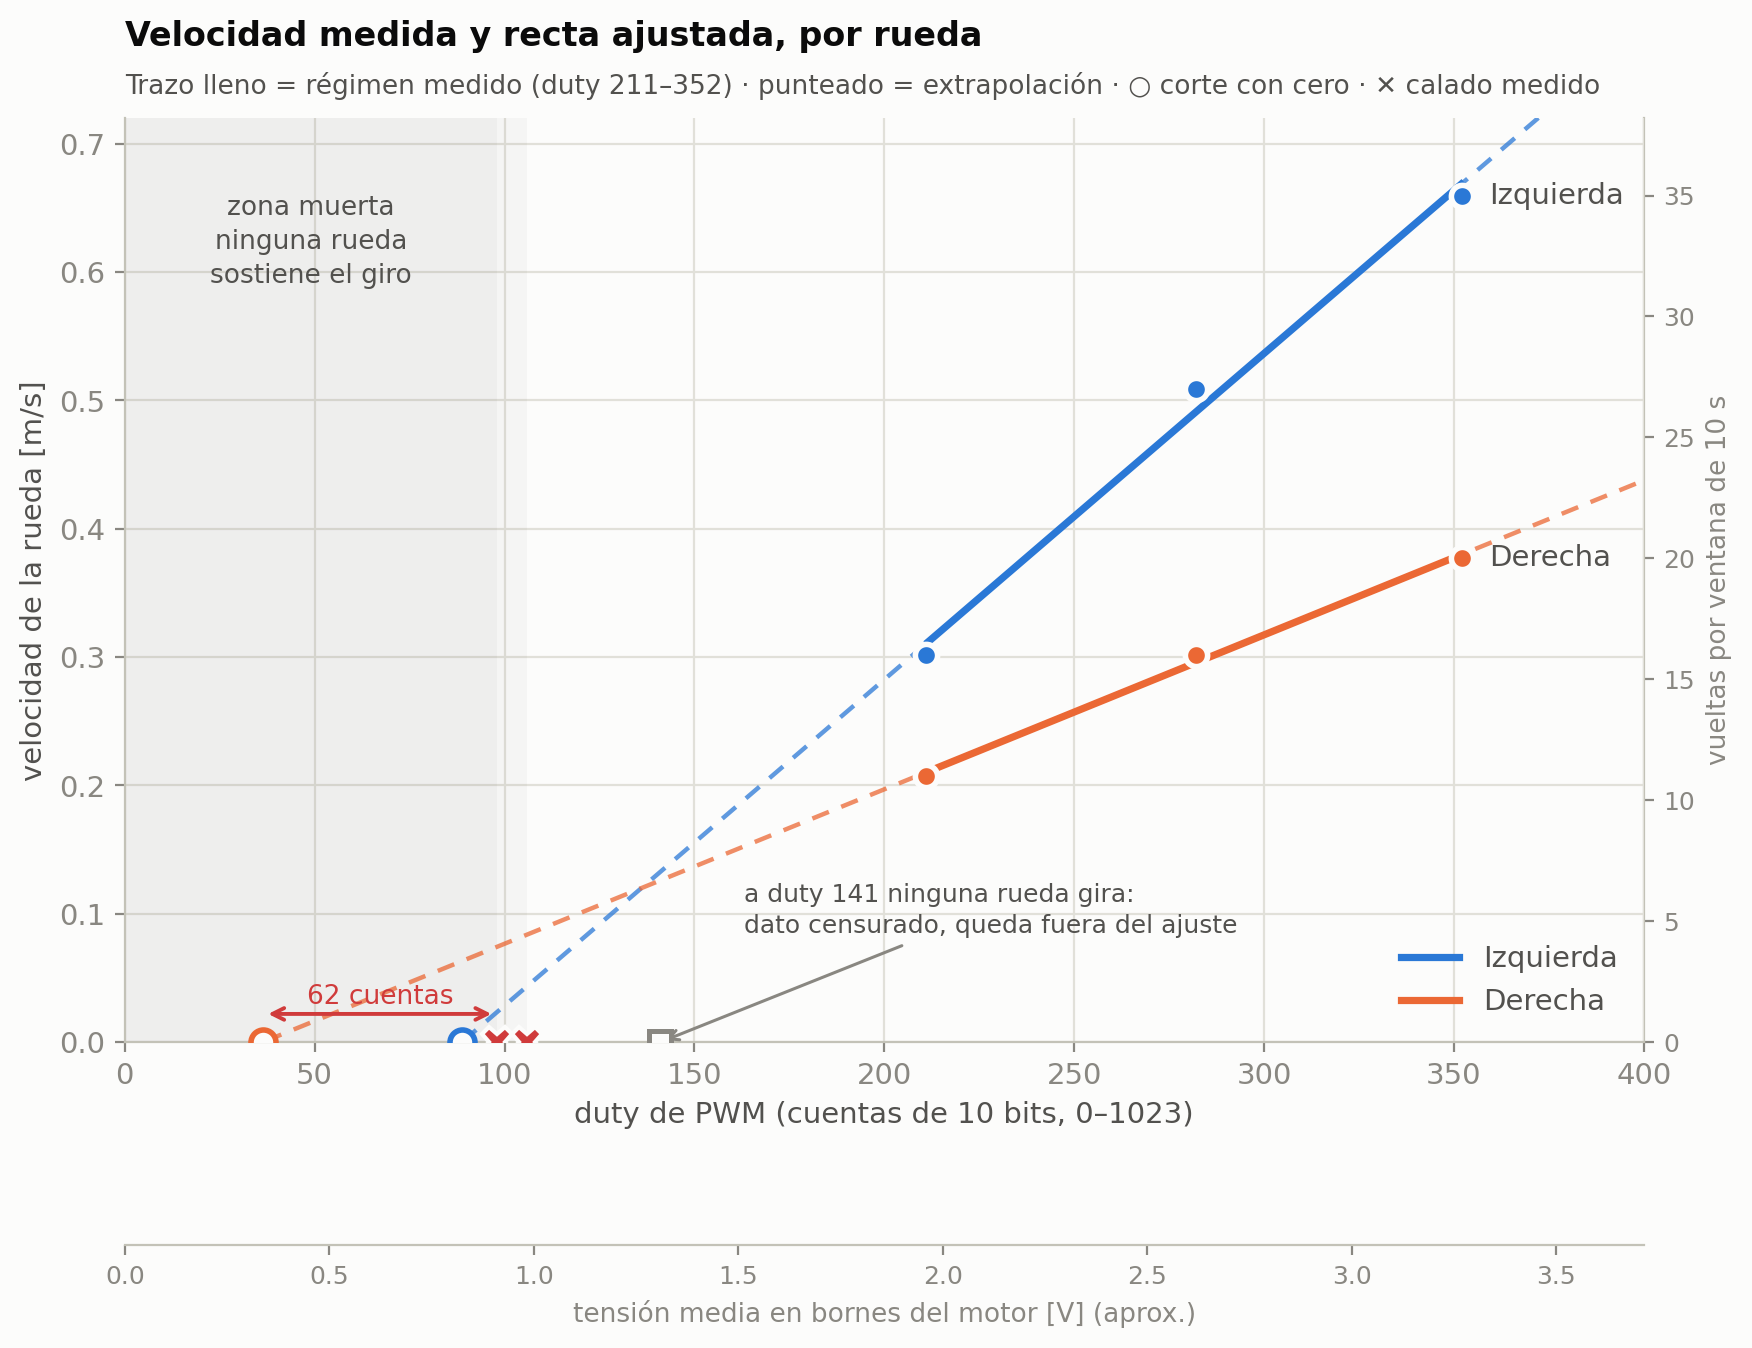
\includegraphics[height=0.25\textheight]{calibracion.png}\hspace{0.6em}
  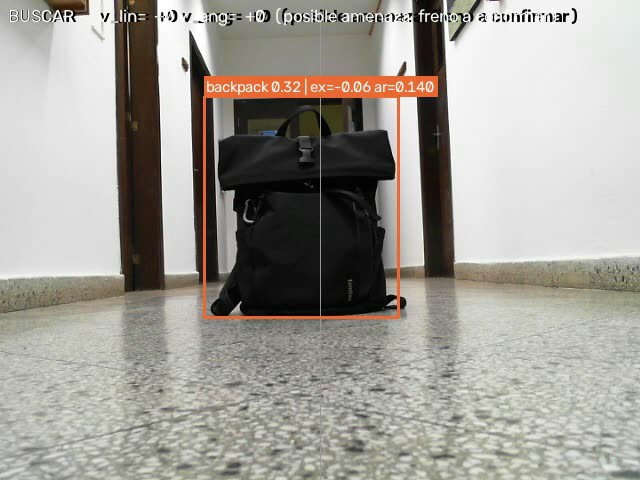
\includegraphics[height=0.25\textheight]{huir_1.jpg}\hspace{0.6em}
  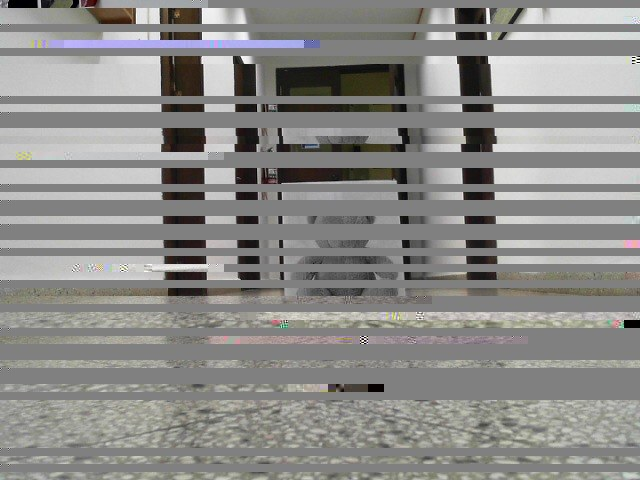
\includegraphics[height=0.25\textheight]{img_rota.jpg}
\end{frame}

% ----------------------------------------------------------------------- 9
\begin{frame}{Resultado: busca el oso, se acerca y frena}
  \begin{columns}[T,onlytextwidth]
    \cuadro{oso_1.jpg}{Busca: no ve nada}
    \cuadro{oso_2.jpg}{Lo ve: se queda quieto y lo confirma}
    \cuadro{oso_3.jpg}{Avanza y lo va centrando}
    \cuadro{oso_4.jpg}{Centrado, frenando}
    \cuadro{oso_5.jpg}{Detenido a $\sim$30 cm}
  \end{columns}

  \vspace{0.8em}
  \begin{columns}[T,onlytextwidth]
    \begin{column}{0.32\textwidth}
      \centering
      {\Large\destaca{13 a 15 s}}\\
      {\small buscando, con el oso a 1 m y a 90\grad}
    \end{column}
    \begin{column}{0.32\textwidth}
      \centering
      {\Large\destaca{0,2 s}}\\
      {\small para confirmarlo desde que lo ve}
    \end{column}
    \begin{column}{0.32\textwidth}
      \centering
      {\Large\destaca{2,5 s}}\\
      {\small de aproximación hasta frenar}
    \end{column}
  \end{columns}

  \vspace{0.6em}
  {\footnotesize\textcolor{grisclaro}{Imágenes de la cámara del robot durante
  una corrida en el piso, con lo que la red detecta.}}
\end{frame}

% ---------------------------------------------------------------------- 10
\begin{frame}{Resultado: ve la mochila y huye}
  \begin{columns}[T,onlytextwidth]
    \cuadro{huir_1.jpg}{La ve y la confirma}
    \cuadro{huir_2.jpg}{Retrocede girando}
    \cuadro{huir_3.jpg}{Gira hasta darle la espalda}
    \cuadro{huir_4.jpg}{Se aleja $\sim$65 cm}
    \begin{column}{0.19\textwidth}
      \centering
      \vspace{0.6em}
      {\Large\textcolor{naranja}{\textbf{0,2 s}}}\\
      {\footnotesize desde que la ve hasta que decide huir}
    \end{column}
  \end{columns}

  \vspace{0.9em}
  \begin{block}{Video: 20 segundos vistos desde el robot}
    Busca el oso y se acerca; después ve la mochila y huye.
    \hfill\cod{demo_vista_del_robot.mp4}
  \end{block}

  \vspace{0.3em}
  \small
  Con la mochila al lado del oso mientras se acercaba, \textbf{huyó}: la
  prioridad se cumple. Y huyendo hacia una pared, el ultrasónico corta el
  avance a \textbf{30 cm} y el robot gira hasta tener el camino libre.
\end{frame}

% ---------------------------------------------------------------------- 11
\begin{frame}{Lo que se midió}
  \small
  \begin{tabular}{L{6.0cm}L{2.8cm}L{4.4cm}}
    \toprule
    & \textbf{Objetivo} & \textbf{Medido} \\
    \midrule
    Imágenes por segundo, lazo completo & 5 o más & \textbf{11} \\
    De la foto a la decisión & --- & $\sim$150 ms \\
    Alcance de detección del oso & --- & $\sim$1,3 m \\
    Distancia de frenado al oso & $\sim$30 cm & alrededor de 30 cm \\
    Reacción ante la mochila & --- & 0,2 s \\
    Distancia a una pared, huyendo & no chocar & corta a 29 cm; mínimo 27 \\
    Freno si el Pi se cuelga & menos de 1 s & menos de 1 s \\
    Alimentación con baterías & sin caídas & sin caídas en 10 corridas \\
    \bottomrule
  \end{tabular}

  \vspace{0.2em}
  \begin{alertblock}{Lo que todavía no hay}
    Son pruebas de \textbf{puesta a punto}, no una evaluación estadística.
    Falta la serie de 10 corridas por escenario para dar porcentajes de éxito.
  \end{alertblock}
\end{frame}

% ---------------------------------------------------------------------- 12
\begin{frame}{La lección del trabajo}
  \begin{alertblock}{}
    \centering\large
    Un número vale \textbf{en el contexto donde se midió}.
  \end{alertblock}

  \vspace{0.5em}
  \begin{columns}[T,onlytextwidth]
    \begin{column}{0.32\textwidth}
      \begin{block}{La calibración}
        \small Exacta con las ruedas al aire. En el piso, una rueda no
        arrancaba.
      \end{block}
    \end{column}
    \begin{column}{0.32\textwidth}
      \begin{block}{La velocidad de giro}
        \small 165\grad{} por segundo, medida en varias vueltas. En un giro de
        un segundo dio unos 110\grad.
      \end{block}
    \end{column}
    \begin{column}{0.32\textwidth}
      \begin{block}{La etiqueta}
        \small ``Mochila'' es correcta para las fotos del entrenamiento. Desde
        el piso, es ``valija''.
      \end{block}
    \end{column}
  \end{columns}

  \vspace{0.6em}
  \small
  Pasó \textbf{21 veces}, del integrado de potencia a la red neuronal. La
  respuesta de método: anotar al lado de cada número \textbf{en qué
  condiciones se midió}, y probar una capa por vez.
\end{frame}

% ---------------------------------------------------------------------- 13
\begin{frame}{Límites y trabajo futuro}
  \begin{columns}[T,onlytextwidth]
    \begin{column}{0.485\textwidth}
      \begin{alertblock}{Límites de esta versión}
        \begin{itemize}
          \item \textbf{Sólo ve obstáculos adelante}: retrocede y gira a
                ciegas.
          \item Reconoce el oso hasta $\sim$1,3 m.
          \item La imagen USB falló de a ratos, sin causa aislada.
          \item Falta la evaluación con series de corridas.
        \end{itemize}
      \end{alertblock}
    \end{column}
    \begin{column}{0.485\textwidth}
      \begin{block}{Segunda versión}
        \begin{itemize}
          \item \textbf{Sensores atrás y a los costados}: hoy retrocede y
                gira sin ver.
          \item \textbf{Encoders}: lazo de velocidad por rueda.
          \item Más alcance: imagen más grande sólo mientras busca.
        \end{itemize}
      \end{block}
    \end{column}
  \end{columns}

  \vspace{0.6em}
  \small
  Lo que queda demostrado: \destaca{percepción con IA, decisión y actuación,
  cerradas en un robot físico, en tiempo real y a bordo}.
\end{frame}

% ---------------------------------------------------------------------- 14
\begin{frame}[standout]
  Gracias

  \vspace{0.6em}
  {\large ¿Preguntas?}
\end{frame}

% =============================================================================
%  Respaldo: no se presentan; están para las preguntas.
% =============================================================================
\appendix
\newcounter{ultimaprincipal}
\setcounter{ultimaprincipal}{\value{framenumber}}

\begin{frame}{Respaldo: los parámetros principales}
  \footnotesize
  \begin{tabular}{L{4.1cm}L{2.4cm}L{6.7cm}}
    \toprule
    \textbf{Parámetro} & \textbf{Valor} & \textbf{De dónde sale} \\
    \midrule
    Tamaño de inferencia & 320 px & Medido: a 640, 3 por segundo; a 320, 11 \\
    Confirmar / perder & 3 / 5 imágenes & Diseño: no reaccionar a una detección aislada \\
    Umbral: oso / mochila & 0,35 / 0,20 & La mochila da 0,32 a 0,41 a 1,2 m \\
    Ganancia de giro & 0,5 & 0,8 se pasaba de largo; 0,3 perdía el oso \\
    Velocidad máxima & 0,25 m/s & Los motores dan 0,87 m/s; la visión no \\
    Área objetivo & 0,35 & Decide frenar a $\sim$38 cm y queda a $\sim$30 \\
    Paso de búsqueda & 0,25 s ($\sim$18\grad) & Medido con la cámara: 35 \% de la imagen \\
    Pausa de búsqueda & 0,6 s & Unas 6 imágenes nítidas por pausa \\
    Huida: atrás, giro, adelante & 1,5 / 1,2 / 2,5 s & Ajustado en el piso \\
    Ultrasónico: esquivar / llegar & 30 / 20 cm & Con 20 solo, al huir quedaba a 11 cm \\
    Freno automático & 500 ms & Sin órdenes del Pi, el ESP32 frena \\
    \bottomrule
  \end{tabular}

  \vspace{0.3em}
  Todos en un solo archivo (\cod{config.py}), cada uno con cómo se midió.
\end{frame}

\begin{frame}{Respaldo: seguridad y protocolo}
  \begin{columns}[T,onlytextwidth]
    \begin{column}{0.485\textwidth}
      \begin{block}{Protocolo: texto, una orden por línea}
        \small
        \cod{M,<avance>,<giro>} \quad de $-100$ a $100$\\
        \cod{B,<patron>} \quad buzzer: alarma o llegada\\
        \cod{D,<distancia>,...} \quad telemetría, 20 por segundo

        \vspace{0.3em}
        El Pi manda \emph{intención}; el ESP32 la convierte en potencia para
        cada rueda con su calibración.
      \end{block}
    \end{column}
    \begin{column}{0.485\textwidth}
      \begin{block}{Tres redes de seguridad}
        \small
        \begin{enumerate}
          \item \textbf{0,4 s}: si la visión se cuelga, el Pi manda ``parar''.
          \item \textbf{0,5 s}: si el Pi deja de hablar, el ESP32 frena solo.
          \item \textbf{La mano}: el conector de 12 V de los motores.
        \end{enumerate}
      \end{block}
    \end{column}
  \end{columns}

  \vspace{0.6em}
  \small
  Las dos primeras se probaron en hardware: dejando el programa vivo pero
  callado, y matándolo. Además, un \textbf{ultrasónico al frente}: con algo a
  menos de 30 cm, no avanza. \ojo{Sólo mira adelante.}
\end{frame}

\begin{frame}{Respaldo: la imagen rota}
  \begin{columns}[c,onlytextwidth]
    \begin{column}{0.36\textwidth}
      \centering
      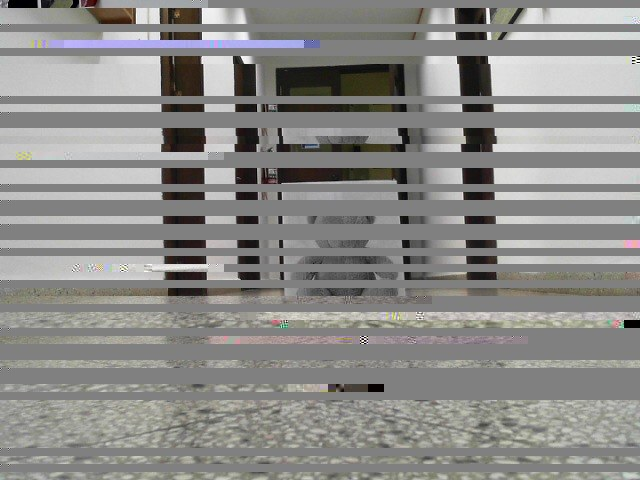
\includegraphics[width=\textwidth]{img_rota.jpg}\\[3pt]
      {\footnotesize Robot quieto, motores desenchufados}
    \end{column}
    \begin{column}{0.61\textwidth}
      \small
      \textbf{Qué pasó:} con el robot quieto, 69 de 71 imágenes llegaron con
      franjas grises. Media hora después, 0 de 606.

      \vspace{0.4em}
      \textbf{Descartado con mediciones:} el ruido de los motores, la fuente
      de 12 V, la carga del procesador, la alimentación del Pi, el ancho de
      banda USB y la cámara en sí.

      \vspace{0.4em}
      \textbf{Lo que se sabe:} son paquetes USB perdidos (lo registra el
      sistema operativo).

      \vspace{0.4em}
      \textbf{Lo que no:} la causa. Al día siguiente, con el enchufe de la
      cámara reinsertado (se había soltado) y las baterías recién cargadas,
      \textbf{0 de 3675}; cambiaron las dos cosas a la vez. Cada corrida mide
      la salud de cada imagen y avisa si la cámara estuvo ``ciega''.
    \end{column}
  \end{columns}
\end{frame}

\begin{frame}{Respaldo: los motores y su calibración}
  \begin{columns}[c,onlytextwidth]
    \begin{column}{0.47\textwidth}
      \centering
      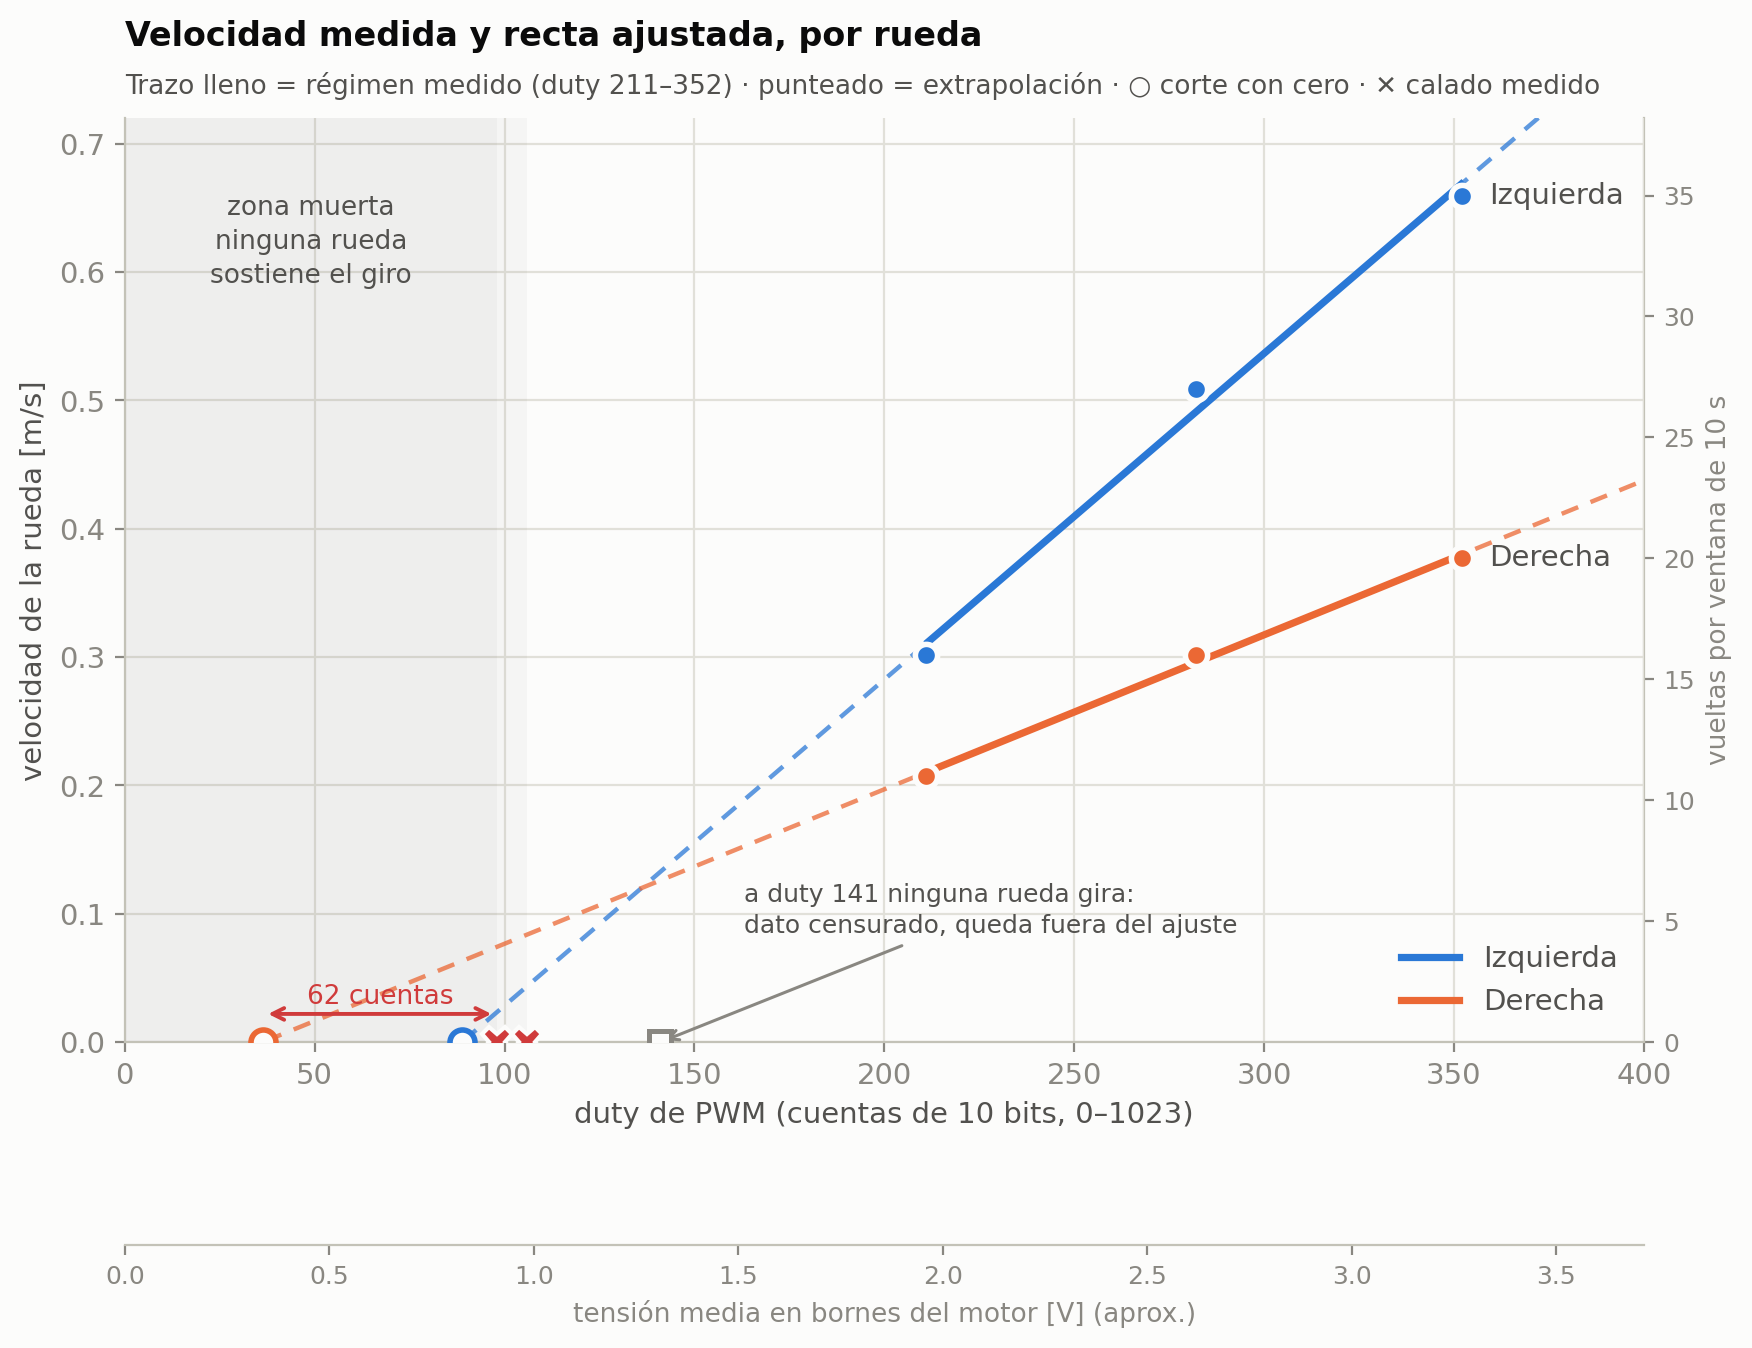
\includegraphics[width=\textwidth]{calibracion.png}
    \end{column}
    \begin{column}{0.50\textwidth}
      \small
      \begin{itemize}
        \item Los dos motores tienen \textbf{reducciones distintas}: uno da
              2,1 veces más velocidad por unidad de potencia.
        \item Solución: \textbf{una recta por rueda}, con piso y techo
              propios. Las dos ruedas siguen la misma velocidad con menos de
              1 \% de diferencia.
        \item No hay arranque suave: la velocidad mínima es 0,09 m/s.
        \item En el piso hubo que \textbf{recalibrar}: la carga suma un
              escalón de potencia y no cambia la pendiente.
      \end{itemize}
    \end{column}
  \end{columns}
\end{frame}

\begin{frame}{Respaldo: cómo se trabajó}
  \small
  \begin{columns}[T,onlytextwidth]
    \begin{column}{0.485\textwidth}
      \begin{block}{Quince jornadas}
        \begin{itemize}
          \item Julio: mecánica y primer movimiento.
          \item Agosto: firmware y calibración de motores.
          \item Septiembre: Raspberry Pi, visión, comportamiento, baterías.
          \item 30/09 y 01/10: \textbf{en el piso}.
          \item 02/10: ultrasónico y buzzer.
        \end{itemize}
      \end{block}
    \end{column}
    \begin{column}{0.485\textwidth}
      \begin{block}{Método}
        \begin{itemize}
          \item Las capas que \textbf{deciden} no tocan hardware: se prueban
                en la PC.
          \item Cada corrida deja un registro, cuadro por cuadro, con sus
                parámetros.
          \item En el piso, \textbf{una capa por vez}, y cada prueba con
                motores anunciada de antemano.
        \end{itemize}
      \end{block}
    \end{column}
  \end{columns}

  \vspace{0.5em}
  Todo está documentado: plan y bitácora, análisis de hardware, guía de
  operación y un resumen técnico de 121 diapositivas.
\end{frame}

\setcounter{framenumber}{\value{ultimaprincipal}}

\end{document}
